\chapter{Provoz}
\label{ch:provoz}

Následující kapitola shrne možnosti realizovaného rozšíření pro koordinaci IoT, popíše, jaké je použití pro provoz
sítě internetu věcí a poté ověří realizované prostředky pro koordinaci IoT na produkčním příkladu.

\section{Nasazení a provoz systému}\label{sec:nasazení-a-provoz-systému}
Pro běh systému s~realizovaným rozšířením bylo nutné zajistit následující prostředky:
\begin{itemize}
    \item \textbf{Server} \\
    Pro běh požadovaných komponent celého systému je požadován server, ke kterému budou schopny se uzly pomocí
    bezdrátové sítě připojit a bude schopen provozovat běhové prostředí Node.js -- v~použitém příkladu se bude jednat
    o~VPS s~operačním systémem Debian.

    \item \textbf{Běhové prostředí pro nástroj Node-RED} \\
    Vzhledem k~ekosystému nástroje Node-RED byl zvolen nástroj PM2\footnote{\url{http://pm2.keymetrics.io/}}, který pro
    aplikace v~programovacím jazyce Javascript zajišťuje správu jejich běhu, tj. monitorování použitých systémových
    prostředků, jejich programové smyčky událostí či paralelní běh -- pro správce systému poskytuje možnost Node-RED
    spustit.

    \item \textbf{Broker MQTT} \\
    Jako broker byla zvolena implementace s~názvem \emph{Eclipse Mosquitto}\footnote{\url{https://mosquitto.org/}} --
    jedná se o~nástroj s~otevřeným zdrojovým kódem od společnosti Eclipse.
    Broker dle dokumentace podporuje všechny z~požadovaných vlastností (parametr zprávy \uv{retain}, tři úrovně QoS,
    zprávu poslední vůle atd.) a je dostupný jako aplikační balíček pro použitý operační systém.

    \item \textbf{Moduly ESP32} \\
    Pro produkční použití byly použity moduly ESP32 s~deskou plošných spojů obsahující stabilizátor napětí, převodník
    UART-USB a lištu pinů umožňující zapojení do nepájivého pole -- jedná se o~moduly s~produktovým názvem
    \uv{ESP32-DevKitC}\footnote{\url{https://www.espressif.com/en/products/hardware/esp32-devkitc/overview}}
    přímo od firmy Espressif Systems.

    \item \textbf{}
\end{itemize}

Všechny výše uvedené prostředky jsem použil pro sestavení vlastního lokálního Internetu věcí, nad kterým jsem následně
prováděl experimenty a ověřoval funkci realizovaných prostředků.
Postup spuštění toto systému byl následující:
\begin{enumerate}
    \item \textbf{Instalace firmwaru na uzel} \\
    Pro realizované programové vybavení pro uzly ESP32 existuje také instalátor v~podobě předpisu pro standardní
    utilitu \texttt{make} -- instalace je složena ze tří hlavních kroků (více k~tomuto postupu je uvedeno v~příloze
    \ref{ch:instalator}).
    Prvním krokem je zavedení samotného interpretu jazyka MicroPython, následuje instalace externích knihoven jakožto
    závislostí realizovaného firmwaru a následně samotný kód firmwaru.
    Po ověření funkce firmwaru je posledním krokem zapnutí automatického zavedení firmwaru při startu -- uzel je v~tu
    chvíli připraven pro provoz čistě přes internetové připojení.
    Výstupem instalace je, kromě pro provoz připraveného uzlu, unikátní identifikátor uzlu, který bude následně použit
    pro zacílení ze strany nástroje Node-RED.

    \item \textbf{Instalace Node-RED rozšíření} \\
    Pro instalaci vlastního rozšíření do tohoto nástroje je nutné dodržet požadavky popsané
    v~\ref{sec:node-red-rozsireni} -- realizované rozšíření všechny tyto formální požadavky splňuje, je tedy možné jej
    nainstalovat do jmenného prostoru knihoven nástroje Node-RED, například pomocí nástroje \texttt{npm}.
    Ve chvíli startu si tento nástroj knihovny poskytující bloky zaregistruje do galerie bloků, které následně nabízí
    uživateli.

    \item \textbf{Příprava sítě} \\
    Dalším krokem je příprava samotné sítě v~nástroji Node-RED, jedná se o~postupně o~výběr bloků pro síť (senzory,
    rozhodovací prvky, výstupní prvky), jejich nastavení (použité piny na uzlu, podmínky, rozmístění prvků v~GUI)
    včetně konfiguračních bloků (broker MQTT, identifikace uzlů získané při instalaci) a na závěr jejich propojení do
    sítě pomocí datových spojů.
    Příklad sítě, která s~pomocí senzoru DHT měří teplotu a vlhkost místnosti, kterou
    exportuje do uživatelského rozhraní, je vyobrazen na obrázku~\ref{fig:node-red-production-1}
    Proces přípravy sítě je zakončen jejím nasazením -- editor zašle konfiguraci do běhové části nástroje, jenž provede
    reinicializaci sítě a jejích bloků.
\end{enumerate}

\todo{vysledky mereni}
\missingfigure{Fotka z~nasazeneho systemu?}

\begin{figure}
    \centering
    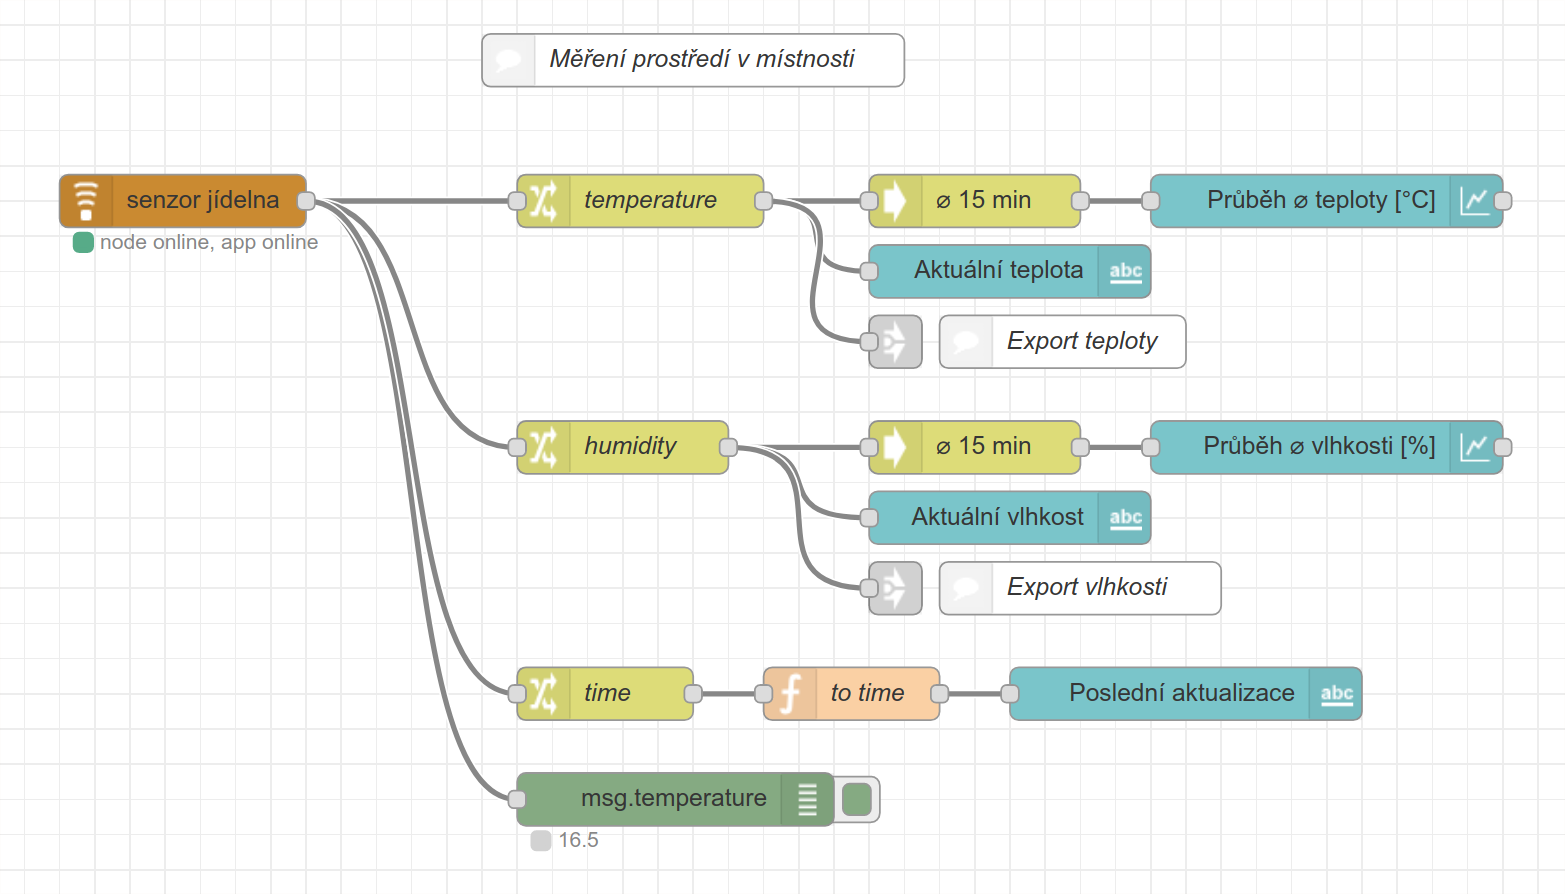
\includegraphics[width=\textwidth]{figures/fis-flow-1.png}
    \caption{Síť z~produkčního nasazení nástroje Node-RED s~realizovaných rozšířením -- vlevo se nachází vstupní blok
    reprezentující uzel s~připojeným senzorem typu DHT22. }
    \label{fig:node-red-production-1}
\end{figure}

\section{Produkční sítě}\label{sec:site-nástroje-node-red}
\missingfigure{screenshot z~nasazene site}
